% =============================================================================
%  s02a-abelian.tex —— §2 阿贝尔陈--西蒙斯理论（引言、2.1、2.2）
%  覆盖原文 p.3（"The theory of Chern and Simons."）— p.9（"CS theory is really
%  good at doing this."）
%  编号公式 (2.1)--(2.19)，图 1（fig:universe），脚注 1、2
% =============================================================================

% ==== 原文 p.3 ====
\section{阿贝尔陈--西蒙斯理论}\label{sec:2}

% [Tutor Note: 本节重点] 物理图像 / 数学工具 / 主要结论 三条
\begin{keytakeaways}
\begin{itemize}[leftmargin=1.4em,itemsep=2pt,topsep=2pt]
  \item \textbf{物理图像：} 3 维 $\mathrm{U}(1)$ 陈--西蒙斯项对 $A$ 是一阶的，没有传播自由度；电荷自带磁通 $\rho=\frac{k}{2\pi}B$，绕电荷一周即得阿哈罗诺夫–玻姆相位，双次交换给出任意子相位 $e^{2\pi i/k}$。
  \item \textbf{数学工具：} 运动方程 $F=0$ 即平坦联络；库仑规范下的解 \eqref{eq:2.7} 是纯规范；高斯环绕积分 $\Phi[\gamma_1,\gamma_2]$ 把威尔逊圈期望值写成环绕数的指数，见 \eqref{eq:2.19}。
  \item \textbf{主要结论：} 大规范变换使 $S_{\mathrm{CS}}\to S_{\mathrm{CS}}+2\pi k$，量子化要求 $k\in\Z$；$\langle W_1W_2\rangle=\exp\!\left(\frac{2\pi i}{k}\Phi\right)$ 表明 CS 理论在计算纽结的环绕数。
\end{itemize}
\end{keytakeaways}

\paragraph{陈与西蒙斯的理论} % 原文标题：The theory of Chern and Simons.
我们不必一头扎进抽象形式，先看一个简单而有教益的例子。设 3 维闵可夫斯基空间 $M=\R^{2,1}$ 代表宇宙。阿贝尔陈--西蒙斯作用量由 $\mathrm{U}(1)$ 规范场 $A_\mu(x)$ 构造，它类似电动力学中的光子场：
\begin{equation}\tag{2.1}\label{eq:2.1}
  S_{\mathrm{CS}}[A] \equiv \frac{k}{4\pi}\int_M \dd^3x\,\varepsilon^{\mu\nu\rho}A_\mu\partial_\nu A_\rho .
\end{equation}

% ==== 原文 p.4 ====
其中 $\varepsilon^{\mu\nu\rho}$ 是全反对称符号，$k\in\R$ 称为陈--西蒙斯能级（level），因子 $\frac{1}{4\pi}$ 纯属约定。这个作用量有点古怪：它只在 3 维才有意义，而且对 $A$ 的导数是一阶的。为了对其行为建立直觉，我们来考察它所定义的理论的经典后果与量子后果。

我们跟随 Dunne 的综述 \cite{dunne}，偶尔借重 Tong 的洞见 \cite{tong_gauge,tong_qhe}。

\subsection{经典理论}\label{sec:2.1}

\paragraph{运动方程} % 原文标题：The equations of motion.
由作用量 \eqref{eq:2.1} 得出的运动方程是
\begin{equation}\tag{2.2}\label{eq:2.2}
  \delta S_{\mathrm{CS}} = 0 \;\Longrightarrow\; \frac{k}{4\pi}\varepsilon^{\mu\nu\rho}F_{\nu\rho} = 0
  \;\Longrightarrow\; F = 0, \qquad F_{\mu\nu} = \partial_\mu A_\nu - \partial_\nu A_\mu .
\end{equation}
这显得相当乏味：没有传播的局部自由度，常数 $k$ 也不影响经典物理。加入物质可以补救。例如，狄拉克费米子 $\psi$ 通过一个流与 CS 项耦合：
\begin{equation}\tag{2.3}\label{eq:2.3}
  \mathcal{L} = \frac{k}{4\pi}\varepsilon^{\mu\nu\rho}A_\mu\partial_\nu A_\rho
  + \bar{\psi}\left(i\not\partial - m\right)\psi
  - eA_\mu\bar{\psi}\gamma^\mu\psi
  = \mathcal{L}_{\mathrm{CS}} + \mathcal{L}_\psi + A_\mu J^\mu .
\end{equation}
用物质流 $J$ 表示，\eqref{eq:2.3} 给出的 $A$ 的运动方程为
\begin{equation}\tag{2.4}\label{eq:2.4}
  \frac{k}{4\pi}\varepsilon^{\mu\nu\rho}F_{\nu\rho}
  = \frac{k}{2\pi}\varepsilon^{\mu\nu\rho}\partial_\nu A_\rho = J^\mu .
\end{equation}

% [Tutor Note: 易错点] (2.4) 的 4π→2π 来自 F_{νρ} 两项相等，因子 2 不可漏
\begin{yizhu}[易错点]
把 \eqref{eq:2.2} 的 $F_{\nu\rho}=\partial_\nu A_\rho-\partial_\rho A_\nu$ 代入：$\varepsilon^{\mu\nu\rho}F_{\nu\rho}=2\varepsilon^{\mu\nu\rho}\partial_\nu A_\rho$，两项因 $\varepsilon$ 全反对称而相等。这就是 \eqref{eq:2.4} 中 $\frac{k}{4\pi}\to\frac{k}{2\pi}$ 的来源。漏掉因子 2，就与 \eqref{eq:2.2} 的系数 $\frac{k}{4\pi}$ 自相矛盾——那里右端恰为 $F=0$，把这一层掩盖了。
\end{yizhu}

\paragraph{插一段几何} % 原文标题：Geometrical aside.
后文会讲到，$A$ 其实是 $M$ 上某个主 $\mathrm{U}(1)$ 丛上的联络，拉格朗日量是陈--西蒙斯 3 形式 $A\wedge\dd A$ 的倍数。场强 $F=\dd A$ 就是该联络的曲率，于是运动方程 $F=0$ 描写平坦联络。物质流 $J$ 的存在把运动方程改为 $\frac{k}{4\pi}\star F=J$（$\star$ 是霍奇星算子），物质于是在规范丛中引入曲率。奇妙的是，这个曲率可以由时空的一个拓扑不变量测量，而该不变量由 CS 形式构造。这一事实是陈--韦伊理论的起点；在数学家看来，那才是研究 CS 作用量的正路 \cite{chern1974}。

\paragraph{电场与磁场} % 原文标题：Electric and magnetic fields.
场强张量 $F_{\mu\nu}$ 由电场 $\mathbf{E}$ 与磁场 $B$ 组成，二者的定义与麦克斯韦理论完全相同：
\begin{equation}\tag{2.5}\label{eq:2.5}
  E_i \equiv -\partial_i A_0 - \partial_0 A_i, \qquad B \equiv \varepsilon^{ij}\partial_i A_j .
\end{equation}
把物质流 $J^\mu\equiv(\rho,\mathbf{J})$ 写成电荷密度与电流密度，直接验证即知 CS 运动方程的分量形式为
\begin{equation}\tag{2.6}\label{eq:2.6}
  \rho = \frac{k}{2\pi}B, \qquad J^i = \frac{k}{2\pi}\varepsilon^{ij}E_j .
\end{equation}

% [Tutor Note: 易错点] (2.6) 依赖 ε^{0ij}=ε^{ij} 与 ε^{ij0}=+ε^{ij} 的指标约定
\begin{yizhu}[易错点]
由 \eqref{eq:2.4} 的 $\mu=0$ 分量得 $J^0=\frac{k}{2\pi}\varepsilon^{0ij}\partial_iA_j$；要得到 \eqref{eq:2.6} 的 $\rho=\frac{k}{2\pi}B$，必须取 $\varepsilon^{0ij}=+\varepsilon^{ij}$（即 $\varepsilon^{012}=+1$、二维 $\varepsilon^{12}=+1$）。$\mu=i$ 分量还需要 $\varepsilon^{ij0}=+\varepsilon^{ij}$ 与 $\varepsilon^{i0j}=-\varepsilon^{ij}$。换一种升降约定，$J^i$ 里的 $\varepsilon^{ij}E_j$ 会整体变号。
\end{yizhu}

% [Tutor Note: 原文疑误] (2.5) 的 E_i 与 (2.6) 的 ε^{ij}E_j 仅在 A_0=0 时自洽
\begin{yizhu}[原文疑误]
取纯电场位形 $A_\mu=(A_0(x),0)$：由 \eqref{eq:2.4} 得 $J^1=\frac{k}{2\pi}\varepsilon^{120}\partial_2A_0=+\frac{k}{2\pi}\partial_2A_0$；而 \eqref{eq:2.6} 配 \eqref{eq:2.5} 给出 $J^1=\frac{k}{2\pi}\varepsilon^{12}(-\partial_2A_0)=-\frac{k}{2\pi}\partial_2A_0$，两者差一个符号（$A_0\neq0$ 时一般差 $2\partial_jA_0$ 项）。原文照录。全节随后都取库仑规范 $A_0=0$，故不影响 \eqref{eq:2.7} 以下的结论。
\end{yizhu}

% ==== 原文 p.5 ====
显然 $B$ 由电荷产生，而 $\mathbf{E}$ 是电流的后果：这与电磁学的情形正好相反。图~\ref{fig:universe} 左画出了这一物理图像：运动的电荷在平面内产生 $\mathbf{E}$ 场，它们的 $B$ 场则指向一个虚构的“$z$”方向。（这幅图在霍尔物理中其实与实验相符。）每条磁通线都附着在一个源电荷上，并穿透空间流形。

% [Tutor Note: 物理图像] 电荷自带磁通，所以绕行相位只依赖环绕数
\begin{yizhu}[物理图像]
\eqref{eq:2.6} 的第一式说明电荷与磁通绑定：一个电荷必拖着一束 $B$ 通量。于是“绕过电荷”等价于“绕过一束磁通”，阿哈罗诺夫–玻姆相位只依赖回路绕这束通量的圈数。任意子相位之所以是拓扑量，根源就在这里。
\end{yizhu}

\begin{figure}[htbp]
  \centering
  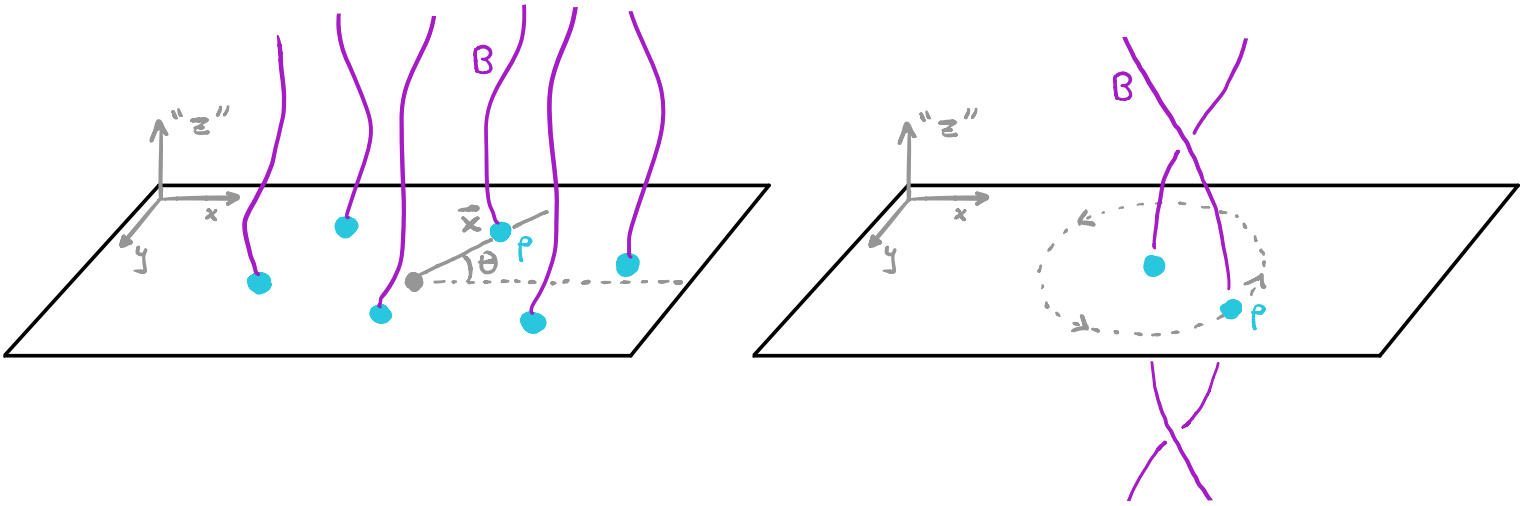
\includegraphics[width=0.95\textwidth]{figures/fig1_cs_universe_anyon.png}
  \caption{左：陈--西蒙斯宇宙。右：一个任意子！（原文 Figure 1，原文 p.5）}
  \label{fig:universe}
\end{figure}

\paragraph{单个检验电荷} % 原文标题：A single test charge.
为了更细致地理解其中的物理，我们来解 CS 方程 \eqref{eq:2.6}，取源为 $\rho=\delta^{(2)}(\mathbf{x}-\mathbf{x}_a(t))$ 与 $\mathbf{J}=\mathbf{0}$。取库仑规范，即 $A_0=0=\partial_iA^i=\nabla\cdot\mathbf{A}$。把这两个源代入 \eqref{eq:2.6}，按 \eqref{eq:2.5} 用 $A_\mu=(0,A_i)$ 写出 $\mathbf{E}$ 与 $B$ 场，再用标准的格林函数技术（具体说，用恒等式 $\nabla^2\log|\mathbf{x}|=2\pi\delta^{(2)}(\mathbf{x})$），即得 \eqref{eq:2.6} 的解：
\begin{equation}\tag{2.7}\label{eq:2.7}
  A_i(\mathbf{x},t) = \frac{1}{k}\varepsilon_{ij}\frac{x^j - x_a^j(t)}{|\mathbf{x}-\mathbf{x}_a|^2}
  = -\frac{1}{k}\partial_i\theta(\mathbf{x}-\mathbf{x}_a(t)),
  \qquad \theta(\mathbf{x}) \equiv \tan^{-1}\!\left(\frac{y}{x}\right) = \arg(\mathbf{x}) .
\end{equation}

% [Tutor Note: 易错点] (2.7) 用下标 ε_{ij}、(2.6) 用上标 ε^{ij}，联立时符号最易出错
\begin{yizhu}[易错点]
取二维 $\varepsilon_{12}=+1$，由 \eqref{eq:2.7} 绕源一周得 $\oint A_i\dd x^i=-2\pi/k$，故 $B=\varepsilon^{ij}\partial_iA_j=-\frac{2\pi}{k}\delta^{(2)}(\mathbf{x}-\mathbf{x}_a)$，代回 \eqref{eq:2.6} 得 $\rho=-\delta^{(2)}$，与正文所取 $+\delta^{(2)}$ 相差一个整体符号。原文照录；凡核对 (2.6) 与 (2.7) 的符号，先固定 $\varepsilon_{12}$ 与 $\varepsilon^{12}$ 的取值，再以 \eqref{eq:2.9} 的 $e^{+i\theta/k}$ 与 \eqref{eq:2.19} 的 $+2\pi i/k$ 为基准。
\end{yizhu}

% [Tutor Note: 含糊点] “standard Green's function techniques” 跳过二维库仑格林函数的构造
\begin{yizhu}[含糊点]
作者省略的求解链条是：由 \eqref{eq:2.6} 与点源得 $\varepsilon^{ij}\partial_iA_j=\frac{2\pi}{k}\delta^{(2)}(\mathbf{x}-\mathbf{x}_a)$，而 $\partial_j\log|\mathbf{x}|=x^j/|\mathbf{x}|^2$，故取 $A_i=\frac{1}{k}\varepsilon_{ij}\partial_j\log|\mathbf{x}-\mathbf{x}_a|$ 即得 \eqref{eq:2.7}。所用定理是二维库仑格林函数恒等式 $\nabla^2\log|\mathbf{x}|=2\pi\delta^{(2)}(\mathbf{x})$（三维对照式 $\nabla^2\frac{1}{|\mathbf{x}|}=-4\pi\delta^{(3)}(\mathbf{x})$），见原文 [10]。
\end{yizhu}

注意 $A_i$ 是全导数：它是纯规范位形。取规范参数 $\omega(\mathbf{x})\equiv\left(\frac{1}{k}\right)\theta(\mathbf{x}-\mathbf{x}_a(t))$，相应的规范变换加上 $\omega$ 的全导数，就把它化为零。于是 $A(x)\equiv0$，$\mathbf{E}\equiv\mathbf{0}$、$B=0$ 都成了平凡结论。但同一个规范变换也作用在物质场 $\psi$ 上——它正是源电荷的载体——给它一个非平凡的阿哈罗诺夫–玻姆相位，该相位取决于角位置 $\theta$ 与 $k$：
\begin{equation}\tag{2.8}\label{eq:2.8}
  \omega = \frac{1}{k}\theta \;\Longrightarrow\;
  \begin{cases}
    A_i(x) \longrightarrow A'(x) = A_i(x) + \partial_i\omega(x) = 0,\\[2pt]
    \psi(x) \longrightarrow \psi'(x) = e^{i\omega(x)}\psi(x) = e^{i\theta/k}\psi(x).
  \end{cases}
\end{equation}

% [Tutor Note: 原文疑误] (2.8) 首行 A'(x) 漏掉下标 i
\begin{yizhu}[原文疑误]
\eqref{eq:2.8} 首行左端是 $A_i(x)$，右端却写 $A'(x)$ 无下标，同一行的 $A_i(x)+\partial_i\omega(x)$ 又带下标 $i$。按下标一致性应读作 $A'_i(x)$。原文字面照录，译文不改。
\end{yizhu}

% [Tutor Note: 原文疑误] p.5 “Aharanov-Bohm” 应为 Aharonov–Bohm
\begin{yizhu}[原文疑误]
原文 p.5 此处拼作 “Aharanov-Bohm”，标准拼写是 Aharonov–Bohm（阿哈罗诺夫–玻姆）。属拼写笔误，译文按规范术语处理，原文拼写照录于此。
\end{yizhu}

\paragraph{双次交换与任意子} % 原文标题：Double exchange and anyons.
现在考虑两个电荷，如图~\ref{fig:universe} 右。一个保持静止，另一个绕它运动。我们把这一过程看作双次交换：运动的电荷与静止的电荷交换位置两次，每转 $\pi$ 一次。

% ==== 原文 p.6 ====
由 \eqref{eq:2.8}，运动粒子得到的相位为
\begin{equation}\tag{2.9}\label{eq:2.9}
  \Delta\theta = 2\pi \;\Longrightarrow\;
  \psi(x) \longrightarrow \exp\!\left(\frac{2\pi i}{k}\right)\psi(x)
  = \exp\!\left(i\oint_{\theta=0}^{\theta=2\pi}\dd x^i A_i\right)\psi(x) \neq \psi(x) .
\end{equation}

% [Tutor Note: 含糊点] (2.9) 末端的 ψ(x)≠ψ(x) 左右同一记号
\begin{yizhu}[含糊点]
\eqref{eq:2.9} 末端写作 $\psi(x)\neq\psi(x)$，两边记号相同，因为原文对变换后的场仍写 $\psi(x)$（\eqref{eq:2.8} 里写的是 $\psi'(x)$）。读时应把右端理解为 $\psi'(x)$：绕行一周后波函数只差一个相位，不是同一个态。相位 $\exp(2\pi i/k)$ 正是 \eqref{eq:2.8} 第二式取 $\theta=2\pi$ 的结果。
\end{yizhu}

若这些粒子是玻色子或费米子，$\psi$ 在双次交换后会回到自身。但 \eqref{eq:2.9} 表明，调节 $k$ 就能赋予 $\psi$ 取值于 $\mathrm{U}(1)$ 的任意统计。所以这些粒子是任意子，因为它们可以有任意统计。（量 $e^{2\pi i/k}$ 与 $A$ 的闭合回路积分的指数式，会在本综述中反复出现。）

\paragraph{几点评论} % 原文标题：Comments.
任意子得到的相位只依赖 $k$ 与所走路径的拓扑。在我们的例子里，它绕静止电荷在 $\R^2$ 上扎出的一个穿孔点转了一圈（该点处电荷为无穷大）。可见 CS 理论自带一个场论探针——任意子相位——它能探测 $\R^2\backslash\{\mathbf{0}\}\simeq S^1\times\R$ 中非平凡回路的绕数。同一想法的另一个反映，是图~\ref{fig:universe} 中磁通线的缠绕。下面会看到，把这些磁通线看成在无穷远处闭合的回路——也就是纽结——很有用。这一视角不仅给出高斯定律的一幅图像，还揭示出 CS 理论实际上在计算这些 $B$ 场纽结的环绕数。要点在于：CS 理论没有局部自由度，却强烈影响相距很远的粒子，并且知道红外物理 \cite{tong_gauge}。

\subsection{路径积分量子化}\label{sec:2.2}

\paragraph{规范不变吗？} % 原文标题：Gauge invariance?
讨论任意子时，我们已经看到 CS 理论在规范变换下的性质。现在转向一个更简单也更基本的问题：我们要证明纯 CS 作用量 \eqref{eq:2.1} 不是规范不变的。这个项目一开始就极不顺利：在形如 $A_\mu\to A'_\mu=A_\mu+\partial_\mu\omega$ 的规范变换下，计算表明作用量改变一个全导数：
\begin{equation}\tag{2.10}\label{eq:2.10}
  S_{\mathrm{CS}} \longrightarrow S'_{\mathrm{CS}} = S_{\mathrm{CS}}
  + \frac{k}{4\pi}\int_M \dd^3x\,\varepsilon^{\mu\nu\rho}\partial_\mu(\omega\,\partial_\nu A_\rho) .
\end{equation}
若 $\omega$ 在无穷远处为零，边界项为零，$S_{\mathrm{CS}}$ 就规范不变。尴尬的是，即使 $\omega$ 在无穷远处不为零，只要没有磁单极子，由高斯定律，阿贝尔 CS 作用量仍然规范不变。\footnote{正如我们将看到的，非阿贝尔理论并非如此，它更脆弱：所有“大”规范变换（large gauge transformation）都使作用量发生非平凡变换，无需向理论中添加磁单极子。由此得到的变换 $S_{\mathrm{CS}}\to S_{\mathrm{CS}}+2\pi k$，与带磁单极子的阿贝尔理论相同。} 因此我们来描写磁通破坏规范不变性的最简单情形。最终，一个精心挑选的规范变换会让作用量按 $S_{\mathrm{CS}}\to S_{\mathrm{CS}}+2\pi k$ 变换。下面会看到，这意味着在量子理论中 $k$ 必须是整数。

% [Tutor Note: 含糊点] “由高斯定律仍规范不变”一句跳过了边界项为零的论证
\begin{yizhu}[含糊点]
这句“即使 $\omega$ 在无穷远处不为零……仍然规范不变”没有给证明。由 \eqref{eq:2.10}，$\delta S_{\mathrm{CS}}=\frac{k}{4\pi}\int_M\dd^3x\,\partial_\mu(\omega\varepsilon^{\mu\nu\rho}\partial_\nu A_\rho)$ 是全导数的积分，化为空间无穷远 $S^2$ 上的通量 $\oint_{S^2}\omega\,B\,\dd S$。没有磁单极子时 $\oint_{S^2}B\,\dd S=0$（高斯定律，斯托克斯定理的直接推论），故为零。下一段正是靠“引入磁通”打破这一零。见原文 [10]。
\end{yizhu}

% ==== 原文 p.7 ====
\paragraph{欧氏空间的杂技} % 原文标题：Euclidean acrobatics.
要打破 $S_{\mathrm{CS}}$ 的规范不变性，最省事的办法是把空间流形紧致化为 $S^2$，再经威克转动 $t\to\tau=it$ 转到欧氏号差，时间轴 $\R$ 于是变成热圆周 $S^1$。关键在于，CS 作用量对时间导数是一阶的，它变换为 $S_{\mathrm{CS}}\to S^{\mathrm{E}}_{\mathrm{CS}}=-iS_{\mathrm{CS}}$。接着选规范变换 $\omega(\tau,\mathbf{x})=\frac{2\pi\tau}{\beta}$，它绕热圆周转一整圈，不能连续形变为恒等映射。最后引入磁通，即 $B=F_{12}$ 在 $S^2$ 上的非零积分。为此设想 $S^2\subset\R^3$ 包围一个安放在原点的磁单极子，再测穿过其表面的通量。念及狄拉克，我们回想起 $\mathrm{U}(1)$ 的紧致性使这类通量量子化：
\begin{equation}\tag{2.11}\label{eq:2.11}
  \int_{S^2} F_{12} = 2\pi n, \qquad n\in\Z .
\end{equation}
至此，全部配料齐备：考虑 $M=S^2\times S^1$ 上的规范变换 \eqref{eq:2.10}，代入上面给出的 $\omega$。分部积分表明，边界项正比于上面的通量积分；取 $n=1$，得 $\delta S_{\mathrm{CS}}=2\pi k$。

% [Tutor Note: 含糊点] 从 (2.10) 到 δS_CS=2πk 的中间步骤全被 “proportional” 一句带过
\begin{yizhu}[含糊点]
作者只写“边界项正比于通量积分”。把 \eqref{eq:2.10} 与 \eqref{eq:2.11} 的字面量代入：$\delta S_{\mathrm{CS}}=\frac{k}{4\pi}\cdot\frac{2\pi}{\beta}\cdot\beta\cdot2\pi n=\pi kn$，取 $n=1$ 得 $\pi k$；正文写作 $2\pi k$，两者差因子 2，差异只能落在 $\omega$ 的绕数或磁单极荷的归一化上。此处照录原文 $2\pi k$，并与 \eqref{eq:2.12} 的 $e^{2\pi ik}=1$ 一并核对。
\end{yizhu}

\paragraph{配分函数} % 原文标题：The partition function.
看来麻烦不小：$S_{\mathrm{CS}}$ 并不规范不变！但只要配分函数 $\mathcal{Z}$ 规范不变，量子理论仍有救。联立 $\delta S_{\mathrm{CS}}=2\pi k$ 与 $-S^{\mathrm{E}}_{\mathrm{CS}}=iS_{\mathrm{CS}}$，$\mathcal{Z}$ 的路径积分变换如下：
\begin{equation}\tag{2.12}\label{eq:2.12}
  \mathcal{Z} = \int\mathcal{D}A\,e^{-S^{\mathrm{E}}_{\mathrm{CS}}}
  \longrightarrow \int\mathcal{D}A\,e^{i(S_{\mathrm{CS}}+2\pi k)}
  = \int\mathcal{D}A\,e^{2\pi ik}e^{-S^{\mathrm{E}}_{\mathrm{CS}}}
  = e^{2\pi ik}\mathcal{Z} .
\end{equation}
幸亏 $S_{\mathrm{CS}}$ 与所有拓扑项一样，在欧氏号差下是虚的；只要 CS 能级 $k$ 是整数，路径积分就规范不变。

\paragraph{任意子即威尔逊圈} % 原文标题：Anyons as Wilson loops.
我们已经用路径积分量子化了 CS 能级，现在再用它从更形式的视角重新发现任意子，做法依波利亚科夫 \cite{polyakov1988}。回到洛伦兹号差，考虑纯 CS 理论的生成泛函，即有源 $J$ 时的配分函数：
\begin{equation}\tag{2.13}\label{eq:2.13}
  \mathcal{Z}[J] \equiv \frac{1}{\mathcal{Z}}\int\mathcal{D}A\,\exp\left[i\int_M \dd^3x\left(\frac{k}{4\pi}\varepsilon^{\mu\nu\rho}A_\mu\partial_\nu A_\rho + A_\mu J^\mu\right)\right]
  \equiv \frac{1}{\mathcal{Z}}\int\mathcal{D}A\,e^{i\widetilde{S}_{\mathrm{CS}}[A,J]} .
\end{equation}

% [Tutor Note: 易错点] (2.13) 的 1/𝒵 归一化：𝒵 同时指配分函数与生成泛函
\begin{yizhu}[易错点]
同一字母 $\mathcal{Z}$ 既作配分函数 \eqref{eq:2.12}，又作生成泛函 $\mathcal{Z}[J]$。\eqref{eq:2.13} 前面的 $1/\mathcal{Z}$ 使 $\mathcal{Z}[J=0]=1$，于是 \eqref{eq:2.16} 的“$\equiv\langle W_1W_2\rangle$”自动成立，不必再除一次 $\mathcal{Z}$；若按惯例定义 $\mathcal{Z}[J]\equiv\int\mathcal{D}A\,e^{iS+i\int A J}$，则 \eqref{eq:2.16} 应写成 $\mathcal{Z}[J]=\mathcal{Z}\langle W_1W_2\rangle$。两种写法只差整体归一化，不影响 \eqref{eq:2.19} 的相位。
\end{yizhu}

为了复现图~\ref{fig:universe} 中的物理情形，考虑两个粒子在平面内沿闭合回路 $\gamma_1$、$\gamma_2$ 互相绕行。用源 $J\equiv J_1+J_2$ 描写它们，其中
\begin{equation}\tag{2.14}\label{eq:2.14}
  J_a^\mu \equiv \oint_{\gamma_a}\dd x_a^\mu\,\delta^{(3)}(x-x_a(t)), \qquad a\in\{1,2\} .
\end{equation}

% ==== 原文 p.8 ====
借这些“点电荷”$\delta$ 函数，作用量里的源项等于
\begin{equation}\tag{2.15}\label{eq:2.15}
  \int_M \dd^3x\,A_\mu J^\mu = \oint_{\gamma_1}\dd x_1^\mu\,A_\mu + \oint_{\gamma_2}\dd x_2^\mu\,A_\mu .
\end{equation}
我们认出，\eqref{eq:2.15} 里这些源的指数式就是所谓的威尔逊圈，它是非局域可观测量，定义为 $W_a\equiv\exp\left[i\oint_{\gamma_a}\dd x_a^\mu A_\mu\right]$。（它们不过是 \eqref{eq:2.9} 的任意子相位换了装！）

% [Tutor Note: 原文疑误] p.8 “anyonic phass” 应为 “anyonic phase”
\begin{yizhu}[原文疑误]
原文此句作 “the anyonic phass (2.9)”，拼写有误，应为 “anyonic phase”；对照 p.6 的 “the anyonic phase” 可确认。译文按 phase 处理，原文拼写照录于此。
\end{yizhu}

用 $W_1$、$W_2$ 表示，路径积分 \eqref{eq:2.13} 变成二者乘积的期望值：
\begin{equation}\tag{2.16}\label{eq:2.16}
  \begin{aligned}
  \mathcal{Z}[J] &= \frac{1}{\mathcal{Z}}\int\mathcal{D}A\,\exp\left[i\oint_{\gamma_1}\dd x_1^\mu A_\mu\right]\exp\left[i\oint_{\gamma_2}\dd x_2^\mu A_\mu\right]e^{iS_{\mathrm{CS}}[A]} = \\
  &= \frac{1}{\mathcal{Z}}\int\mathcal{D}A\,W_1W_2\,e^{iS_{\mathrm{CS}}} \equiv \langle W_1W_2\rangle .
  \end{aligned}
\end{equation}

\paragraph{环绕数} % 原文标题：The linking number.
因为有源 CS 作用量 $\widetilde{S}_{\mathrm{CS}}[A,J]$ 对 $A$ 是二次的，路径积分 \eqref{eq:2.13} 是高斯型。于是把经典解 $A_\mu^{\mathrm{cl}}$ 代入 \eqref{eq:2.16}，就能精确算出它（相差一个无关的归一化常数）。我们已在库仑规范中求出过这个解，但在洛伦兹规范中做一遍也有用：\footnote{这一步非常微妙。在洛伦兹规范中，CS 运动方程 \eqref{eq:2.4} 化为平坦 4 维时空 $\R^{3,1}$ 中标准的（麦克斯韦）静电学方程。按 \eqref{eq:2.17} 的记号，希腊指标 $\mu$、$\nu$、$\rho$ 是 $\R^{3,1}$ 的\emph{空间}指标，而 $x$、$y$ 等视为 $\R^3$ 中的（空间）矢量。因此量 $|x-y|$ 是要我们计算 $x$ 与 $y$ 在 $\R^3$ 中的欧氏距离。}
\begin{equation}\tag{2.17}\label{eq:2.17}
  A_\mu^{\mathrm{cl}}(x) = \frac{1}{2k}\int_M \dd^3y\,\varepsilon_{\mu\nu\rho}\frac{\partial^\nu J^\rho(y)}{|x-y|}
  = \frac{1}{2k}\sum_{a=1}^{2}\oint_{\gamma_a}\dd x_a^\nu\,\varepsilon_{\mu\nu\rho}\frac{(x-x_a)^\rho}{|x-x_a|^3} .
\end{equation}
这里代入了 \eqref{eq:2.14} 的 $J$，并做了分部积分。接着把 \eqref{eq:2.17} 的解代入 $\widetilde{S}_{\mathrm{CS}}$。由于对 $A$ 二次，有源作用量由两条回路 $\gamma_a$ 上的两重积分构成；这一事实抓住了两个（局域）粒子间相互作用的非局域本性。同一条回路上积分两次的项是发散的：它们描写自相互作用，即使 $J$ 只描写单个粒子也存在。

把 \eqref{eq:2.17} 代入 \eqref{eq:2.16}，去掉自相互作用项（或把它们并入归一化常数），做完代数，得到
\begin{equation}\tag{2.18}\label{eq:2.18}
  \mathcal{Z}[J] = \langle W_1W_2\rangle = \exp\left(i\widetilde{S}_{\mathrm{CS}}[A^{\mathrm{cl}}]\right)
  = \exp\left(\frac{i}{2k}\oint_{\gamma_1}\dd x_1^\mu\oint_{\gamma_2}\dd x_2^\nu\,\varepsilon_{\mu\nu\rho}\frac{(x_1-x_2)^\rho}{|x_1-x_2|^3}\right).
\end{equation}

% [Tutor Note: 含糊点] “去掉自相互作用项（或并入归一化常数）”一句跳过了正规化
\begin{yizhu}[含糊点]
把 \eqref{eq:2.17} 代入后，$\gamma_a$ 与自身的双重积分在 $x_1=x_2$ 处发散，对应自环绕数 $\Phi[\gamma_a,\gamma_a]$。作者一句“或并入归一化常数”带过：实际做法是先承认该项发散、照 \eqref{eq:2.18} 只保留 $\gamma_1\neq\gamma_2$ 的互作用项，再以配分函数之比定义期望值。自环绕数要等 \S\ref{sec:3} 引入标架化才有定义，参见原文 [6]。
\end{yizhu}

指数上的积分与一个称为高斯环绕积分的量有关：
\begin{equation}\tag{2.19}\label{eq:2.19}
  \Phi[\gamma_1,\gamma_2] \equiv \frac{1}{4\pi}\oint_{\gamma_1}\dd x_1^\mu\oint_{\gamma_2}\dd x_2^\nu\,\varepsilon_{\mu\nu\rho}\frac{(x_1-x_2)^\rho}{|x_1-x_2|^3}
  \;\Longrightarrow\;
  \langle W_1W_2\rangle = \exp\left(\frac{2\pi i}{k}\Phi[\gamma_1,\gamma_2]\right).
\end{equation}
高斯证明 $\Phi[\gamma_1,\gamma_2]$ 是整数，并且是个拓扑不变量，称为 $\gamma_1$ 与 $\gamma_2$ 的环绕数，它数一条曲线绕另一条缠绕的次数。

% ==== 原文 p.9 ====
取 $\Phi=1$ 就回到 \eqref{eq:2.9} 得到的任意子相位 $\langle W_1W_2\rangle=e^{2\pi i/k}$。

\paragraph{解读} % 原文标题：Interpretation.
图~\ref{fig:universe} 为这段数学故事提供了两幅漂亮的实现。第一，高斯积分对学过电动力学的人并不陌生：$\Phi[\gamma_1,\gamma_2]$ 计算单匝线圈因穿过它的电流回路而收到的磁通 \cite{ricca2011}。而且把线圈与电流回路互换，$\Phi$ 不变：$\Phi[\gamma_1,\gamma_2]=\Phi[\gamma_2,\gamma_1]$。在 CS 理论中这一点有用：从源电荷伸出的磁通线彼此穿过对方的通量，正比于它们纠缠的程度；这又探测了电荷本身的任意子交换相位。第二，注意 $\Phi$ 的被积函数是高斯映射 $\Gamma:(x_1,x_2)\mapsto\frac{x_1-x_2}{|x_1-x_2|}$ 的雅可比行列式；该映射把 $\gamma_1$、$\gamma_2$ 投影到单位球面 $S^2\subset\R^3$，并识别出它们的“交叉”点。把磁通线投影到平面，就是高斯映射本身的直观表示；其行列式甚至出现在经典解 \eqref{eq:2.7} 与 \eqref{eq:2.17} 中。所以环绕积分登场，也不必太感意外。

这里的要点是：威尔逊圈计算纽结的拓扑不变量，而这些不变量又是物理可观测量。下面就会看到，CS 理论做这件事真的很在行。

% =============================================================================
% 【片段汇报】sections/s02a-abelian.tex
% 覆盖：原文 p.3–p.9（§2 标题与引言、2.1 经典理论、2.2 路径积分量子化）
% 编号公式：19 个，(2.1)–(2.19)，逐条对照 work/pages/p03–p09.png 核过
% 图：1 幅（fig:universe，原文 Figure 1，p.5）
% 脚注：2 条（p.6 脚注 1、p.8 脚注 2）
% 译注：14 条（易错点 4、含糊点 5、物理图像 1、原文疑误 4）+ 本节重点 1 框
% 原文笔误（均照录并批注）：
%   1. p.8 “anyonic phass” → phase（已核页面图像，确为 phass）
%   2. p.5 “Aharanov-Bohm” → Aharonov–Bohm
%   3. p.5 式 (2.8) 首行 A'(x) 漏下标 i（左端 A_i、同行 A_i+∂_iω 均带 i）
%   4. p.4 式 (2.5) 的 E_i 与 (2.6) 的 ε^{ij}E_j 仅在 A_0=0 时自洽（A_0≠0 时差 2∂_jA_0）
% 存疑：
%   1. p.7 δS_CS=2πk：按 (2.10)+(2.11) 字面代入得 πkn（n=1 即 πk），与正文 2πk
%      差因子 2；未改正文，仅在译注中提示核对。
%   2. p.5 (2.6) 与 (2.7) 联立：若取二维 ε^{12}=ε_{12}=+1，则源为 −δ^{(2)}，
%      与正文所取 +δ^{(2)} 差一整体符号；已在译注中说明，未改正文。
%   3. 正文引用 \S\ref{sec:3}（标架化），须确认 s03a-framing.tex 定义了 \label{sec:3}。
% =============================================================================
